\documentclass[tikz]{standalone}
\usepackage{amsmath}
\definecolor{bg}{HTML}{171D2B}
\definecolor{ak}{HTML}{F7B538}
\begin{document}
\pagecolor{bg}
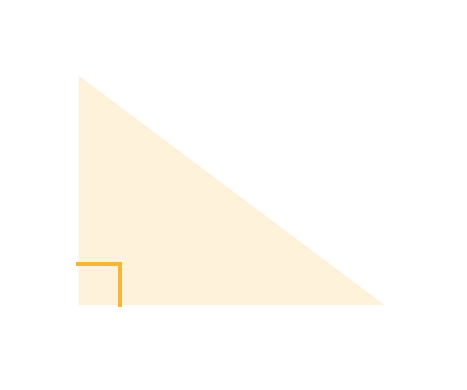
\begin{tikzpicture}[line width=1.6pt,
  every node/.style={text=white, font=\large}]
  % Segitiga siku-siku 3-4-5, siku di C
  \coordinate (C) at (0,0);
  \coordinate (A) at (0,3);
  \coordinate (B) at (4,0);
  \draw[white, fill=ak!18] (C) -- (A) -- (B) -- cycle;
  % penanda siku
  \draw[ak, line width=1.4pt] (0.55,0) -- (0.55,0.55) -- (0,0.55);
  % label titik
  \node[above left]  at (A) {$A$};
  \node[below right] at (B) {$B$};
  \node[below left]  at (C) {$C$};
  % label sisi
  \node[left=4pt]  at (0,1.5) {$a$};
  \node[below=4pt] at (2,0)   {$b$};
  \node[above right=2pt] at (2,1.5) {$c$};
\end{tikzpicture}
\end{document}
